\section{Motivation}
\label{sec:motivation}

%We motivate our work by describing the current practice in network
%configuration. In traditional networks with distributed control planes, the operators' goal is to generate the configuration of individual devices based on their desired policy. This configuration dictates the behavior of a device, how it exchanges routing information with neighbors and how it filters and ranks that information. The collective behavior of the devices should implement the desired policy.
%
%Device configuration languages are low-level and indirect. For instance, instead of allowing operators to express directly the paths they want through the network, they require operators to specify metrics that result in those paths; instead of allowing operators to express directly the types of traffic to not carry through the network, they require operators to select and program an appropriate filtering mechanism (e.g., BGP import or export filters, null routing,  access control lists) and instantiate it on topologically appropriate devices; instead of allowing operators to directly specify that they prefer BGP neighbors in a certain order, they require operators to program local preferences and multi-exit discriminators (MED) at each router and ensure that the numbers are consistent across routers.
%
%In many networks today, device configurations are generated manually by operators, without the support of many automated tools. It is easy to see the problems with this approach, such as typos, inconsistency across devices, and no guarantees of policy compliance.
%
%To reduce such problems, some networks use a template-based approach. Configuration templates abstract certain constants into variables (e.g., instead of concrete community value, they may contain a variable {\small \sf{\$$BadNeighbor$)}} and may use a device vendor-neutral syntax. Operators manually generate the templates and use tools to translate them into device configuration, by replacing variables with appropriate constants using a database of network information.
%
% %and replacing vendor-neutral constructs with their vendor-specific counterparts.
%
%%In practice, most networks use a hybrid of templates and manual generation of device configuration. Templates are used for standardized and common configuration elements across devices and the result is manually tweaked to obtain the exact desired network behavior.
%
%While templates avoids some pitfalls of the fully manual approach, they too are far from ideal. The fundamental issue is the semantic mismatch between desired policies and the level of abstraction of templates. While many policies are network-wide (e.g., prefer customer networks, or never announce a route to a certain prefix to external neighbors), templates are device-level. Operators must still manually decompose network-wide policies into device-level policies that can produce the desired network-wide behavior.
%This decomposition is not always straightforward and ensuring policy-compliance can be hard, especially in the face of failures. We illustrate this point using two examples based on policies that we have seen in practice and we demonstrate the ease with which the
%examples are described using our new language \sysname.

%Operators today generate the BGP configuration of individual devices based on intended policy. 
When generating BGP configurations, whether fully manually or aided by templates, the operators face the challenge of decomposing network-wide policies
into appropriate device-level policies.
This decomposition is not always straightforward and ensuring policy-compliance is tricky, especially in the face of failures. We illustrate this point using two examples based on policies that we have seen in practice. The next section shows how \sysname allows operators to directly express these policies. 
%the ease with which the
%policies can be specified using our new language \sysname.
%The next section describes how to automatically compile this specification to device-level policies.

\subsection{Example 1:  The Backbone}

Consider the backbone network in Figure~\ref{fig:example1}. It has
three neighbors, a customer \CD{Cust}, a peer \CD{Peer}, and a provider \CD{Prov}. The policy of this network is shown on the right. It prefers the neighbors in a certain order (P1) and does not want to act as a transit between \CD{Peer} and \CD{Prov} (P2). It prefers to exchange traffic with \CD{Cust} over \CD{R1} rather than \CD{R2} because \CD{R1} is cheaper (P3). To guard against another AS "hijacking" prefixes owned by \CD{Cust}, it only sends traffic to them if \CD{Cust} is on the AS path (P4). Finally, to guard against \CD{Cust} accidentally becoming a transit for \CD{Prov}, it does not use \CD{Cust} for traffic that will later traverse \CD{Prov} (P5).

To implement P1 of the policy, the operators must compute and assign
local preferences such that preferences at \CD{Cust}-facing interfaces
$>$ \CD{Peer}-facing interfaces $>$ \CD{Prov}-facing interfaces. At
the same time, to satisfy P3 the preference at \CD{R2}'s
\CD{Cust}-facing interface should be lower than that at
\CD{R1}. Implementing P3 properly will require MEDs to be appropriately configured. 
To implement P2, the operators can assign communities that
indicate where a certain routing announcement entered the
network. Then, \CD{R4} must be configured to not announce to
$\CD{Peer}$ routes that have communities that correspond to the
\CD{R2}-\CD{Prov} link but to announce routes with communities for the \CD{R2}-\CD{Cust} and \CD{R1}-\CD{Cust} links. Finally, to implement P4 and P5, the operators will have to compute and configure appropriate prefix- and AS-path-based filters at each router.

Clearly it is no simple task to properly configure even this
small example network manually; devising correct configurations for real networks can quickly become a nightmare. Such networks have many neighbors across multiple commercial-relationship classes, differing numbers of links per neighbor, along with several neighbor- or prefix-based exceptions to the default behavior. For example, a large AS with many peers in different geographic locations may be faced with complex challenges like keeping traffic within national boundaries.
Templates help to an extent by keeping preference and community values consistent across routers, but operators must still do much of the conceptually difficult work manually. 
%\sysname lets operators express such policies easily and intuitively. It then automatically generates per-device import and export filters, local preferences, MED attributes, and community tags to ensure that the policy is implemented correctly under all failure scenarios.


\begin{figure}[t!]
  \centering
  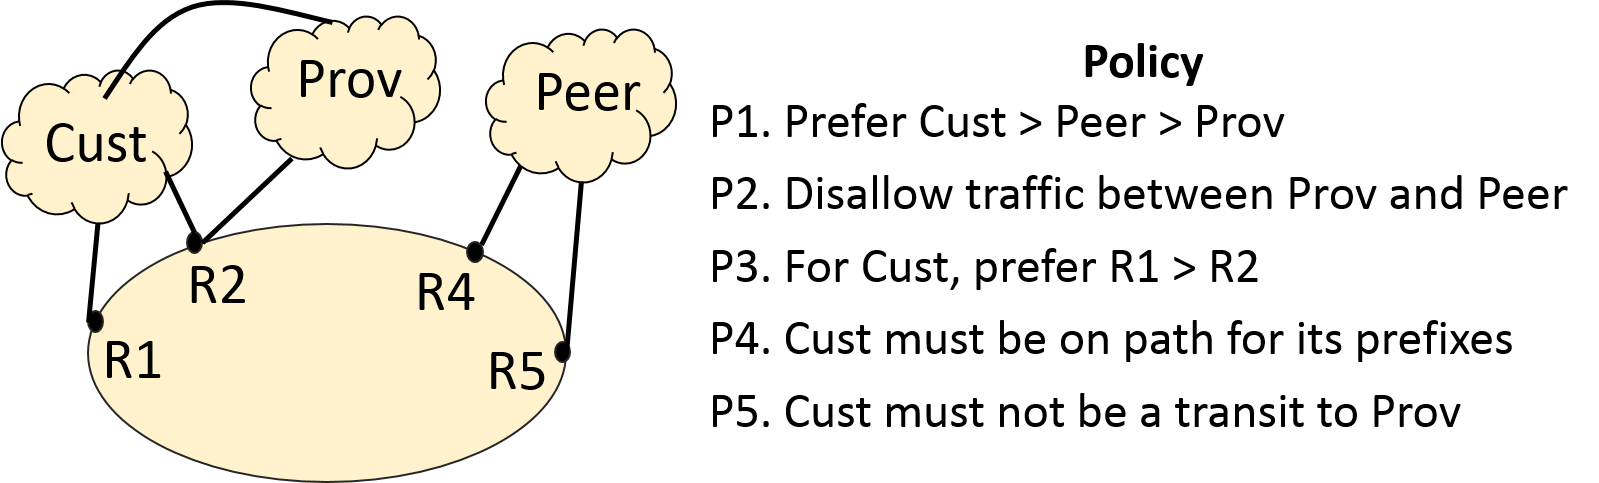
\includegraphics[width=\columnwidth]{figures/example1}
  \caption{Creating router-level policies is difficult.}
  \label{fig:example1}
  \vspace{-1em}
\end{figure}


\subsection{Example 2:  The Data Center}

 While configuring policies for a fully functional network is difficult, ensuring policy compliance in the face of failures can be almost impossible. Consider the data center network in Figure~\ref{fig:example2} with routers organized as a fat tree and running BGP.\footnote{For scale and policy flexibility, data center networks increasingly use BGP internally, with a private AS number per router~\cite{bgp-in-dc}.} The network has two clusters, one with services that should be reachable globally and one with services that should be accessible only internally. This policy is enabled by using non-overlapping address space in the two clusters and ensuring that only the address space for the global services is announced externally. Further, to reduce the number of prefixes that are announced externally, the global space is aggregated into a less-specific prefix \CD{PG}. The semantics of aggregation is that the aggregate prefix is announced as long as the router has a path to at least one sub-prefix.

The operator may decide that a simple way to implement the policy is to have X and Y: $i)$ not export externally what they hear from G and H, routers that belong to the local services cluster; and $ii)$ announce what they hear from routers C and D and aggregate to \CD{PG} if an announcement is subset of \CD{PG}. This implementation is appealing because X and Y do not need to be made aware of which prefixes are global versus local and IP address assignment can be done independently (e.g., new prefixes can be assigned to local services without updating router configurations).

\begin{figure}[t!]
  \centering
  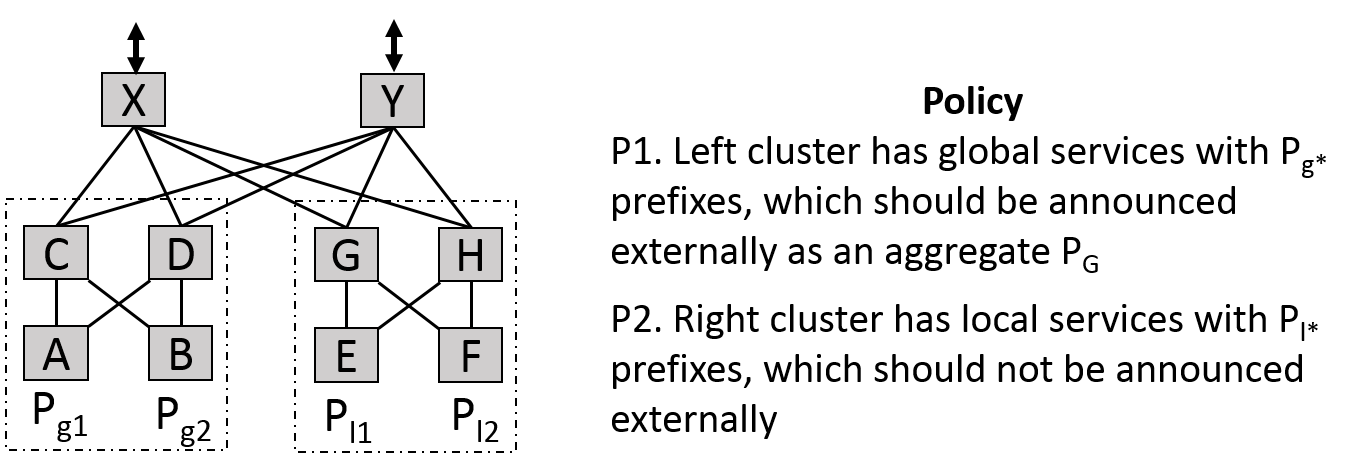
\includegraphics[width=\columnwidth]{figures/example2}
  \caption{Policy-compliance under failures is difficult.}
  \label{fig:example2}
  \vspace{-1em}
\end{figure}

However, this implementation does not have the right behavior in the face of failures. Suppose links X--G and X--H fail. Then, X will hear announcements for \CD{PL*} from C and D, having traversed from G and H to Y to C and D. Per policy implementation, X will start "leaking" these prefixes externally. Depending on the rationale for local services, this leak could impact security (e.g., if the services are sensitive) or availability (e.g., if the \CD{PL*} prefixes are used for other services outside of the data center). This problem does not manifest without failures because then X has and prefers paths to \CD{PL*} through G and H since they are shorter. A similar problem will happen if links Y--G and Y--H fail.
%\footnote{A different problem occurs when links X--C and X--D (or Y--C and Y--D) fail. X (Y) may stop announcing the global prefixes because they would be heard through G and H.}
Link failures in data centers are frequent and it is not uncommon to have multiple failed links at a given time~\cite{dc-failure-study}.

To avoid this problem, the operator may decide to disallow "valley" paths, i.e., those that go up, down, and back up again. This guard can be implemented by $X$ and $Y$ rejecting paths through the other. But that creates a different problem in the face of failures---an aggregation-induced blackhole~\cite{xx}. If links D--A and X--C fail, X will hear announcements for \CD{PG2} from D and will thus announce the \CD{PG} externally. This announcement will bring to X traffic for \CD{PG1} as well, but because of valley-free filtering, X does not have a valid route for \CD{PG1} and will thus drop all traffic to it.

Thus, we see that devising a configuration that ensures policy compliance in the face of failures is complex and error-prone. \sysname lets operators implement their high-level policy specification in a way that guarantees compliance under all failures (if that is possible; otherwise, it generates a compile-time error). For aggregation, it also provides a lower bound to operators on the number of failures under which aggregation will not result in blackholes.



%\subsection{OLD -- Overview}
%\todo{this subsection can be deleted once we have captured everything in it}
%
%Sources of bugs we fix. (It seems like the main advantage of our approach is not just fixing bugs though - it is easily describing high-level intention).
%Perhaps the best way to do this is by going through a bunch of examples in section 2 and showing how you could easily introduce bugs:
%
%\begin{itemize}
%	\item Out of sync, or copy paste errors due to replicated configs (never an issue due to centralized control)
%	\item Correct filtering to ensure no undesired traffic can flow through the network (e.g., best practices, like an AS should filter customers for their prefix, are implemented automatically )
%	\item Failures can easily lead to unexpected behavior (e.g., a datacenter failure scenario w/instability.)
%	\item Trying to do anything interesting, like get backups correct is difficult (e.g., setting up aggregation wrong)
%	\item Related to the last point, things like aggregation can introduce black holes. We have the information needed to prevent this
%\end{itemize}
%
%
%Possible Examples:
%\begin{itemize}
%	\item Basic datacenter with spine preference
%	\item Simple AS that prefers customers over peers over providers
%	\item Combined internal backup routing with preference based entrance into the network using aggregation.
%	\item Something like cold potato routing
%\end{itemize}

